\chapter{Estructura estelar}

Explicar la variada fenomenología descrita en el capítulo anterior ha requerido la solución de retos teóricos en ramas tan variadas como la relatividad general, física de la materia condensada y física nuclear. 

En este capítulo se derivarán las ecuaciones de estructura estelar para una estrella de neutrones fría, neutra, estática y con simetría esférica en la teoría newtoniana y en relatividad general. Después de identificar la necesidad de conocer la EOS de la materia para crear modelos estelares, se  describirá el problema de la EOS de la materia ultradensa y algunos de los métodos usados para hallarla.
%Comparar los dos resultados permitirá identificar algunas de las predicciones de la relatividad general en objetos compactos. 
Para terminar se enunciará una lista de criterios de consistencia física y estabilidad que los modelos estelares deben cumplir, estos criterios serán usados el siguiente capítulo para evaluar qué tan realistas son los modelos estelares obtenidos con diferentes EOSs.




\section{Caso newtoniano}

Considerando una distribución de materia con simetría esférica, si $r$ denota la distancia desde el centro de la configuración, la masa encerrada en una superficie esférica de radio $r$ será:  
\begin{equation}
    m ( r ) = \int _ { 0 } ^ { r } 4 \pi r ^ { 2 } \rho \dd{r} = \int_{0}^{r} \dd{m(r)} \quad\text{con}\quad \dd{m(r)}=4\pi r^2\rho \dd{r},
    \label{mN}
\end{equation}

\begin{equation}
    \Longrightarrow\dv{m(r)}{r} =4\pi r^2 \rho.
    \label{dmnewton}
\end{equation}
Ahora, se considera un cilindro infinitesimal a una distancia $r$ del centro, de altura $\dd{r}$ y sección transversal $\dd{A}$, normal al vector posición $\vec{r}$ (ver Figura \ref{stellnew}).  

\begin{figure}[H]
    \centering
    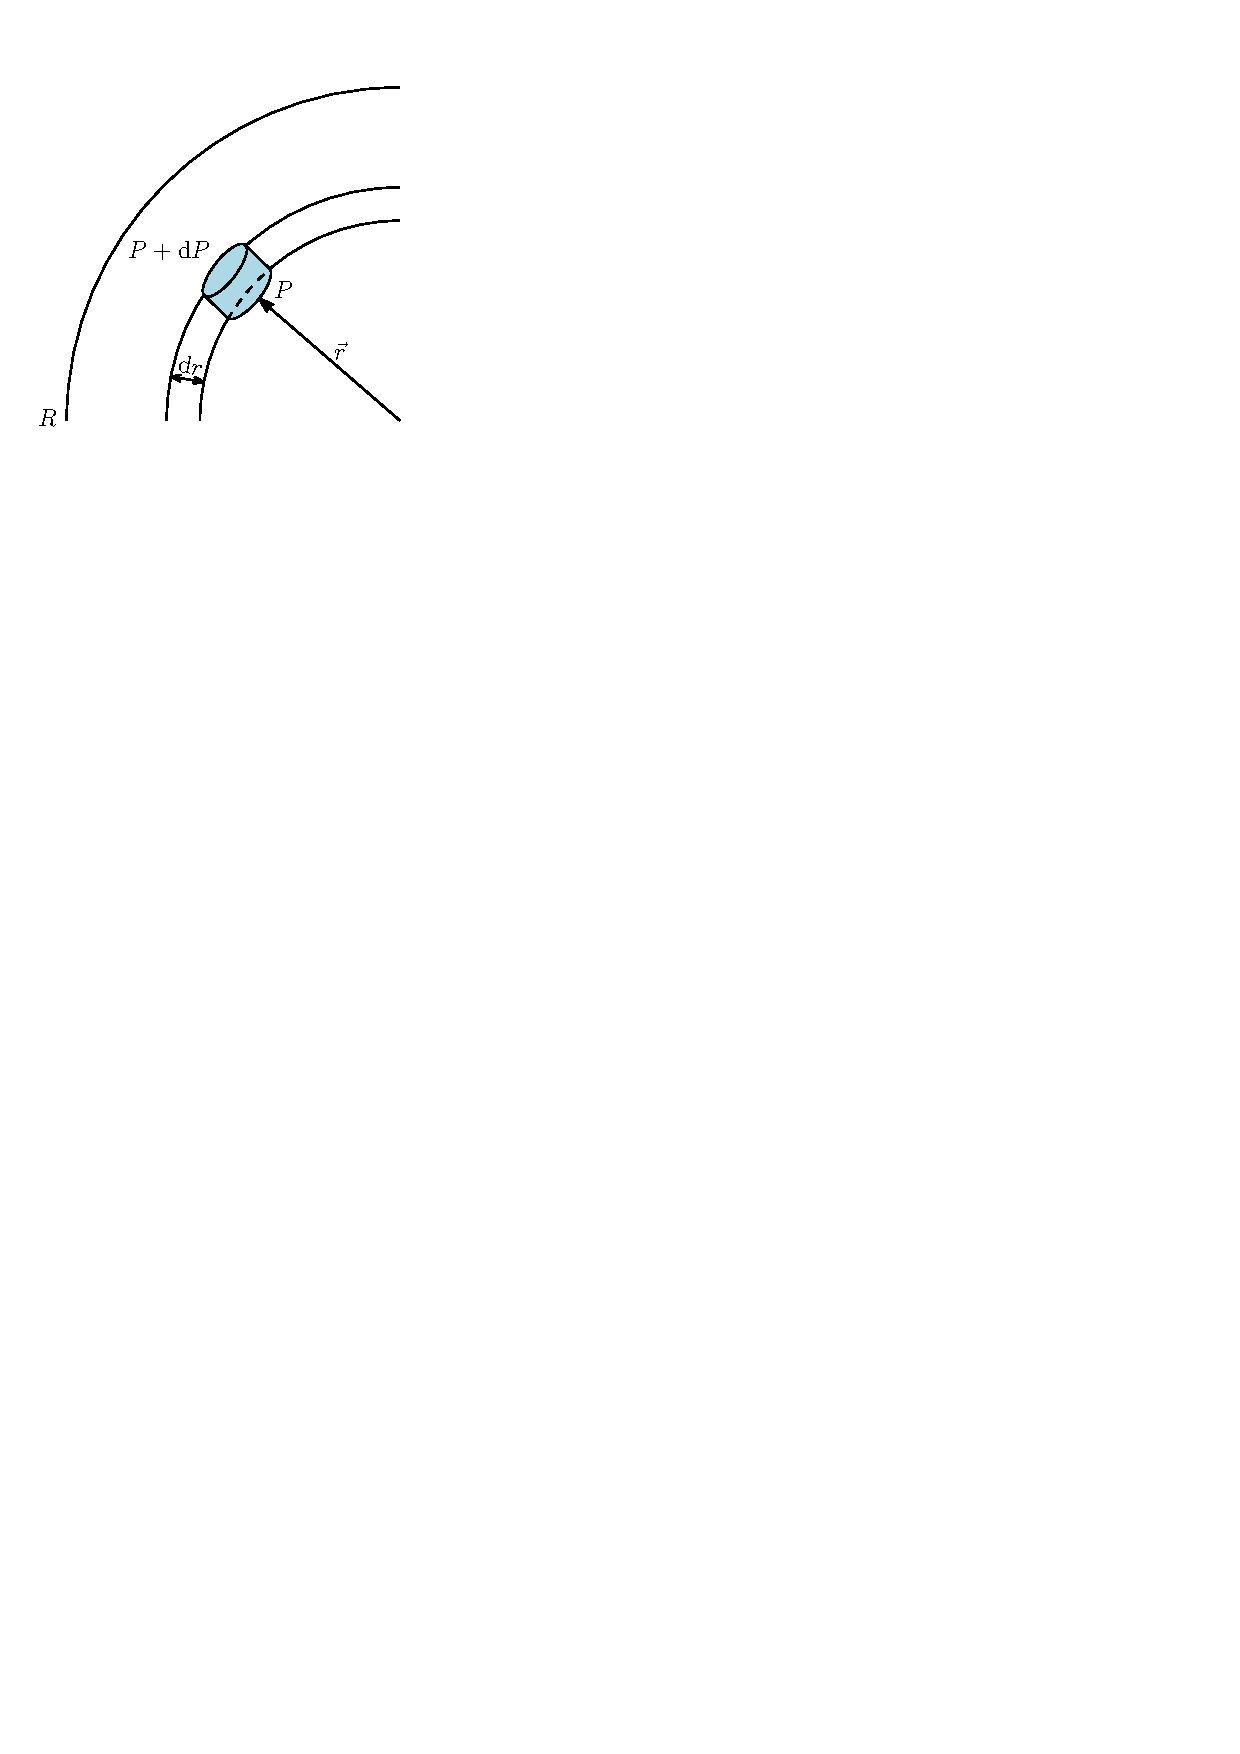
\includegraphics[width=150pt]{figures/stellarnewton.pdf}
    \caption{Presión sobre un elemento de masa cilíndrico.}
    \label{stellnew}
\end{figure}
Si la presión en $\vec{r}$ es $P$ y su cambio al ir de $\vec{r}$ a $\vec{r}+\dd{\vec{r}}$ es $\dd{P}$. La diferencia de presión representa una fuerza 
\begin{equation*}
    F_{Pelem}=-\dd{P}\dd{A},
\end{equation*}
actuando sobre el elemento de masa. Esta fuerza debe contrarrestar la atracción gravitacional sobre el elemento de masa debido a $m(r)$
\begin{equation*}
    F_{atracc}=\frac{G m(r)\rho \dd{A} \dd{r}}{r^2}.
\end{equation*}
Para que el elemento de masa se encuentre en equilibrio se requiere entonces:

\begin{equation}
    -\dd{P}\dd{A} =\frac{G m(r)\rho \dd{A} \dd{r}}{r^2},
\end{equation}
o
\begin{equation}
    \dv{P}{r} = - \frac { G m ( r ) } { r ^ { 2 } } \rho.
    \label{dpnewton}
\end{equation}
que es la conocida ecuación de equilibrio hidrostático. 

Las ecuaciones \eqref{dmnewton} y \eqref{dpnewton} son las ecuaciones de estructura estelar newtonianas \cite{Chandrasekhar1958}. 

%Si una relación entre la presión y la densidad $P(\rho)$ es dada, es decir, una ecuación de estado, el sistema puede resolverse dado un par condiciones iniciales $m(r=0)$ y $P(r=0)$. La primera de estas condiciones es evidente puesto que no hay masa encerrada en un cascarón esférico de radio nulo, $m(r=0)=0$. La segunda estará definida por el valor de $\rho(r=0)\equiv\rho_c$ escogido, mediante la ecuación de estado, $P(r=0)=P(\rho_c)$.

%El radio de la estrella $R$ se define como el valor de $r$ en el que la presión se anula, esto es, $P(R)=0$ y de manera similar la masa de la estrella $M$ se define como el valor de la masa encerrada en $r=R$, esto es, $m(R)=M$.

\REMARK{Decidir si mantener o no} Aunque no se van a tratar en este trabajo, cabe resaltar que las \emph{enanas blancas}, objetos compactos sostenidos por la presión de degeneración de electrones, pueden ser descritas por las ecuaciones de estructura newtonianas satisfactoriamente. Una manera de conocer la importancia de las correcciones relativistas de una estrella es comparando el valor de la compacidad de la estrella $\mu \equiv \frac{2GM}{c^2R}$ con la unidad (la razón será evidente en el resultado relativista) \cite{Weinberg1972}. Las enanas blancas tienen masas en un rango de $0.33\,M_{\odot}$ $1.52\,M_{\odot}$ y radios típicos de unos cuantos miles de kilómetros \cite{Glendenning2000}. Para una enana blanca promedio, con masa $M=0.6\,M_{\odot}$ y radio $r=3000 \,\rm{km}$ se tiene
\begin{equation}
    \mu \simeq 6\times 10^{-4}\ll 1,
\end{equation}
por lo cual se espera que el tratamiento newtoniano sea suficiente. 

\section{Caso relativista}\label{CR}
%\TODO{Basado en los comentarios de la propuesta modificar esta sección. Teniendo en cuenta que los cálculos están hechos en el apéndice.}

%Si bien en la teoría newtoniana podrían existir objetos tan compactos como las estrellas de neutrones, algunas de las predicciones presentan inconsistencias con lo predicho por la teoría de la Relatividad General. Por ejemplo, Chandrasekhar encontró (usando gravedad newtoniana) que las estrellas soportadas por presión de degeneración tienen una masa máxima, obtenida asintóticamente cuando los fermiones son altamente relativistas. Esto es, cuando tienen velocidades comparables con la velocidad de la luz. Bajo tales condiciones la teoría newtoniana permitiría la existencia de estrellas compuestas por los quarks más pesados (charm, bottom y top). En Relatividad General se predice también la existencia de una masa máxima, pero ésta no es de naturaleza asintótica sino que está inmersa en la forma de las ecuaciones de estructura estelar. Las estrellas con la mayor masa posible en Relatividad General, en contraste a lo predicho por la teoría newtoniana, no son lo suficientemente densas para permitir la presencia de los quarks más pesados \cite{Glendenning2000}.

%Predicciones contradictorias como la anterior favorecen a la Relatividad General en el estudio de objetos compactos, pues ésta ha explicado fenómenos como la precesión de mercurio, que no pueden ser explicados en gravedad newtoniana (ver  \cite{Turyshev2008ExperimentalRelativity} para una revisión de tests experimentales de la Relatividad General).

\noindent\small{\textbf{Nota:} a lo largo de esta sección se hará uso de unidades gravitacionales ($G=c=1$), excepto en donde sea explícitamente especificado.}
\normalsize

Para describir la estructura de una estrella estática en Relatividad General se supone un espacio-tiempo asintóticamente plano, estático y con simetría esférica, descrito de manera general por el elemento de linea:

\begin{equation}
\dd{s}^ { 2 } = -e ^ { 2 \nu ( r ) } \dd{ t} ^ { 2 } + e ^ { 2 \lambda ( r ) } \dd{ r} ^ { 2 } + r ^ { 2 } \left( \dd{ \theta} ^ { 2 } + \sin ^ { 2 }  \theta  \dd{ \phi} ^ { 2 } \right) .   
\end{equation}

Respecto a una base ortonormal
\begin{equation}
    \omega^0=\,e^{\nu}\dd{t}, \quad
    \omega^1=\,e^{\lambda}\dd{r}, \quad
    \omega^2=\,r\dd{\theta}, \quad
    \omega^3=\,r\sen{\theta}\dd{\varphi},
\end{equation}
el tensor de Einstein asociado a este elemento de linea tiene componentes no nulas (ver el Apéndice \ref{curvature} para la derivación)

\begin{equation}
    \begin{array} { l } { G _ { 0 } ^ { 0 } = e ^ { - 2 \lambda } \left( \frac { 1 } { r ^ { 2 } } - \frac { 2 \lambda ^ { \prime } } { r } \right) - \frac { 1 } { r ^ { 2 } }  }, \\ { G _ { 1 } ^ { 1 } = e ^ { - 2 \lambda } \left( \frac { 1 } { r ^ { 2 } } + \frac { 2 \nu ^ { \prime } } { r } \right) - \frac { 1 } { r ^ { 2 } } }, \\ { G _ { 2 } ^ { 2 } = e ^ { - 2 \lambda } \left( \nu ^ { \prime \prime } + \nu ^ { \prime 2 } - \lambda ^ { \prime } \nu ^ { \prime } + \frac { \nu ^ { \prime } - \lambda ^ { \prime } } { r } \right)  }, \\ { G _ { 3 } ^ { 3 } = G _ { 2 } ^ { 2 }  }, \end{array}
    \label{eee}
\end{equation}

y debe satisfacer las ecuaciones de Einstein
\begin{equation}
    G _ { \mu } ^ { \nu }  = 8 \pi T _ { \mu } ^ { \nu },
\end{equation}
fijando así las funciones métricas $\nu$ y $\lambda$, en función del contenido material de la estrella descrito por $T _ { \mu } ^ { \nu }$.

Dividiendo el espacio-tiempo en dos: una región exterior a la estrella y una interior. 
La \textit{región exterior} no tiene fuentes ($T _ { \mu } ^ { \nu }=0$) y las ecuaciones de Einstein para ésta son 
\begin{equation}
    G _ { \mu } ^ { \nu } = 0.
\end{equation}
Este es un sistema de 3 ecuaciones, pues $ G _ { 2 } ^ { 2}=G _ { 3 } ^ { 3}$ y dos incógnitas ($\nu$ y $\lambda$). Las identidades de Bianchi aseguran que una las ecuaciones puede ser escrita en términos de las otras y no brinda información adicional.\TODO{Mejorar ese argumento}

Este sistema puede ser resuelto de manera sencilla, restando las dos primeras ecuaciones se obtiene
\begin{equation*}
    G _ { 0 } ^ { 0} - G _ { 1 } ^ { 1} = -e^{-2\lambda} (\nu^{\prime}+\lambda^{\prime}) = 0, 
\end{equation*}
de donde
\begin{align*}
    \nu^{\prime}+\lambda^{\prime} =& \,0 \\
    \int_{r}^{\infty} \qty(\dv{\nu}{r}+\dv{\lambda}{r})\dd{r} =& \,0 \\
    \eval{\nu}_{r}^{\infty} + \eval{\lambda}_{r}^{\infty} =& \, 0,
\end{align*}
como $\lim_{r\to \infty}\nu(r)=\lim_{r\to \infty}\lambda(r)=0$, se llega a que
\begin{equation}
    \nu=-\lambda \quad \Longrightarrow \quad e^{2\nu}=e^{-2\lambda}. \label{metricfsschw}
\end{equation}
Integrando ahora la primera ecuación
\begin{align}
    G _ { 0 } ^ { 0} = -\frac{1}{r^{2}}+e^{-2\lambda}\left(\frac{1}{r^{2}}-\frac{2 \lambda^{\prime}}{r}\right) =& 0 \nonumber \\
    e^{-2\lambda}\left(1-2 \lambda^{\prime} r \right) =& 1 \nonumber \\
    \frac{d\left(r e^{-2 \lambda}\right)}{d r} =& 1 \nonumber \\ 
    r e^{-2 \lambda} =& r - 2 M  \nonumber \\
    e^{2 \lambda} =& \left(1-\frac{2 M}{r}\right)^{-1},
\end{align}
donde $M$ es una constante de integración, que puede ser interpretada como la masa gravitacional al comparar con el límite de campo débil. Finalmente, usando \eqref{metricfsschw} se obtiene
\begin{equation}
    e^{2\nu}=1-\frac{2 M}{r},
\end{equation}

lo que completa la conocida solución exterior de Schwarzschild
\begin{equation}
    \dd{s} ^ { 2 } = - \left( 1 - \frac { 2 M } { r } \right) \dd{t} ^ { 2 } + \left( 1 - \frac { 2 M } { r } \right) ^ { - 1 } \dd{r} ^ { 2 }  + r ^ { 2 } \dd{\theta} ^ { 2 } + r ^ { 2 } \sin ^ { 2 } \theta \dd{\phi} ^ { 2 }, \label{schwarzs}
\end{equation}
valida para $r>R$, donde $R$ es el radio de la estrella. Este elemento de línea describe la geometría del espacio-tiempo exterior a una estrella estática.

Para la \textit{región interior} el contenido material debe ser especificado para resolver las ecuaciones de Einstein. Si la materia se modela como un fluido perfecto, el tensor de energía-momento viene dado por

\begin{equation}\label{EMT}
    \begin{array} { c } { T ^ { \mu \nu } =  P g ^ { \mu \nu } + ( P + \rho ) u ^ { \mu } u ^ { \nu } }, \\ \text{con} \quad { g _ { \mu \nu } u ^ { \mu } u ^ { \nu } = -1 }, \end{array}
\end{equation}
donde $u^{\mu}=\dv{x^{\mu}}{\tau}$ es la cuadri-velocidad de un elemento de fluido, $P$ su presión y $\rho$ su densidad de energía ambas definidas en un marco comóvil con el fluido. Este tensor de energía-momento puede ser deducido del Lagrangiano $L=-\rho$ usando el principio variacional \cite{Felice19992}.

Como se considera una estrella estática, la velocidad espacial de todos los elementos del fluido es cero:
\begin{equation}
    u^{i}=0 \quad (i=1,2,3)\qc u ^ { 0 } = 1
\end{equation}
con lo que las únicas componentes no nulas del tensor energía-momento, en componentes mixtas, serán
\begin{equation}
T _ { 0 } ^ { 0 } = -\rho(r) , \quad T _ { i } ^ { i } =  P(r) \quad ( i=1,2,3 ).  
\end{equation}
Con esta forma del tensor energía-momento y las componentes del tensor de Einstein enunciadas anteriormente, las ecuaciones de Einstein son
\begin{align}
     e ^ { - 2 \lambda } \left( \frac { 1 } { r ^ { 2 } } - \frac { 2 \lambda ^ { \prime } } { r } \right) - \frac { 1 } { r ^ { 2 } } =&  -8\pi\rho, \label{E00} \\
    e ^ { - 2 \lambda } \left( \frac { 1 } { r ^ { 2 } } + \frac { 2 \nu ^ { \prime } } { r } \right) - \frac { 1 } { r ^ { 2 } } =& \, 8\pi P, \label{E11}\\
    e ^ { - 2 \lambda } \left( \nu ^ { \prime \prime } + \nu ^ { \prime 2 } - \lambda ^ { \prime } \nu ^ { \prime } + \frac { \nu ^ { \prime } - \lambda ^ { \prime } } { r } \right) =& \, 8\pi P. \label{E22}
\end{align}

Este sistema de ecuaciones puede ser escrito en una manera más sencilla de integrar usando las Ecuaciones \eqref{E00} y \eqref{E11} suplementadas con la conservación local de la energía y el momento
\begin{equation}
    \qty(\nabla_{\omega_\nu}\mathbf{T})^{\mu \nu} = 0 \label{CEM}.
\end{equation}
La Ecuación \ref{E22} no aportará nueva información pues las identidades de Bianchi aseguran que esta ecuación es una consecuencia de las Ecuaciones \eqref{E00},\eqref{E11} y \eqref{CEM} \cite{Schutz2009}.
 
Reescribiendo la Ecuación \eqref{E00} como
\begin{equation*}
    \dv{\qty[r\qty(1-e^{-2\lambda})]}{r}=8\pi\rho r^2,
\end{equation*}
y definiendo la variable
\begin{equation}
    m(r) \equiv \frac{1}{2}r\qty(1-e^{-2\lambda}) \quad \rightarrow \quad e^{2\lambda} = \qty(1-\frac{2m}{r})^{-1} \label{misnermass} 
\end{equation}
la Ecuación \eqref{E00} en términos de $m$ es simplemente
\begin{equation}
    \dv{m}{r} = 4\pi \rho r^2. \label{dmtov}
\end{equation}

Reescribiendo ahora la Ecuación \eqref{E11} como
\begin{equation*}
    2 r^2 e^{-2\lambda} \nu^{\prime} - r\qty(1- e^{-2\lambda}) = 8\pi P r^3,
\end{equation*}
y usando el cambio de variable \eqref{misnermass}, la Ecuación \eqref{E11} se convierte en 
\begin{equation}
    \dv{\nu}{r}= \frac{m+4\pi P r^3}{r\qty(r-2m)}.\label{dnutov}
\end{equation}

Por último conservación local de la energía requiere
\begin{equation}
      \omega_{\nu} \tensor{T}{^\mu ^\nu} + \tensor{\Gamma}{^\mu _\alpha _\nu}\tensor{T}{^\alpha ^\nu} + \tensor{\Gamma}{^\nu _\alpha _\nu}\tensor{T}{^\mu ^\alpha} = 0,
\end{equation}
donde la conexión $\tensor{\Gamma}{^\alpha _\beta _\gamma}$ (conexión del espín) se relaciona con las 1-formas de conexión \eqref{1fa}, \eqref{1fb}, \eqref{1fc} y \eqref{1fd} mediante
\begin{equation}
    \tensor{\Gamma}{^\alpha _\beta} = \tensor{\Gamma}{^\alpha _\beta _\gamma} \omega^\gamma, \label{covT}
\end{equation}
las componentes de la conexión serán entonces
\begin{align}
        \tensor{\Gamma}{^0_1_0} =& \,\tensor{\Gamma}{^1_0_0} = \nu^{\prime} e^{-\lambda}, \label{sca} \\
        \tensor{\Gamma}{^2_1_2} =& -\tensor{\Gamma}{^1_2_2} = \frac{e^{-\lambda}}{r}, \label{scb} \\
        \tensor{\Gamma}{^3_1_3} =& -\tensor{\Gamma}{^1_3_3} = \frac{e^{-\lambda}}{r}, \label{scc} \\
        \tensor{\Gamma}{^3_2_3} =& -\tensor{\Gamma}{^2_3_3} = \frac{\cot{\theta}}{r} . \label{scd}
    \end{align}
Usando este resultado se encuentra que la única componente que no se anula idénticamente en la Ecuación \eqref{covT} corresponde a $\mu=1$
\begin{align*}
    \omega_{1} \tensor{T}{^1 ^1} + \tensor{\Gamma}{^1 _0 _0}\tensor{T}{^0 ^0} + \tensor{\Gamma}{^1 _i _i}\tensor{T}{^i ^i} + \tensor{\Gamma}{^0 _1 _0}\tensor{T}{^1 ^1} + \tensor{\Gamma}{^i _1 _i}\tensor{T}{^1 ^1} &= 0 \\
    e^{-\lambda} P^{\prime} + \nu^{\prime} e^{-\lambda} \rho -2 \frac{e^{-\lambda}}{r} P + \nu^{\prime} e^{-\lambda} P  + 2\frac{e^{-\lambda}}{r} P  &= 0 \\
    P^{\prime} + (\rho + P) \nu^{\prime} &= 0,
\end{align*}
usando la Ecuación \eqref{dnutov} se obtiene finalmente
\begin{equation}
    \dv{P}{r} = -(P+\rho)\frac{m+4\pi P r^3}{r\qty(r-2m)}.\label{dptov}
\end{equation}

Las ecuaciones \eqref{dmtov}, \eqref{dnutov} y \eqref{dptov} son las ecuaciones de estructura estelar relativista: describen configuraciones de estrellas de neutrones en equilibrio. Este sistema de ecuaciones se conoce generalmente como las ecuaciones de Tolman-Oppenheimer-Volkoff (TOV)  \cite{Tolman1939,Oppenheimer1939} y serán referidas de esta manera en adelante. 

Re-escribiendo \eqref{dptov} en unidades SI como
\begin{equation}
    \dv{P}{r} =  - \frac { G  m ( r ) } { r ^ { 2 } } \rho ( r ) \left[ 1 + \frac { P ( r ) } {c ^ { 2 } \rho ( r ) } \right] \left[ 1 + \frac { 4 \pi r ^ { 3 } P ( r ) } { m ( r ) c ^ { 2 } } \right]  \left[ 1 - \frac { 2 G m ( r ) } { c ^ { 2 } r } \right] ^ { - 1 }, 
    \label{dprelat}
\end{equation}
se aprecia que la versión relativista añade correcciones a la ecuación de equilibrio hidrostático newtoniana \eqref{dpnewton} en forma de tres factores adimensionales. Las dos versiones de las ecuaciones de estructura coinciden cuando estos factores se reducen a la unidad, esto es, en el límite cuando 
\begin{equation}
    c^2\rho \gg P \qc mc^2 \gg 4\pi r^3P \quad \text{y} \quad  \frac{2Gm}{c^2r}= \mu \ll 1,
\end{equation}
en un límite no relativista la variable $m$ definida en \eqref{misnermass} coincide con la masa Newtoniana \eqref{mN}, además $P$ y $\rho$ varían como $\frac{1}{2}mv^2$ y  $mc^2$ \cite{Silbar2003}. Así, las dos primeras correcciones son de orden $v^2/c^2$ y son válidas cuando las partículas del fluido tienen velocidades pequeñas comparadas con la velocidad de la luz mientras el tercer factor es puramente geométrico. 

Debido a que los tres factores en la ecuación \eqref{dprelat} son mayores que 1, si se compararan dos modelos estelares: uno Newtoniano y otro relativista, que para cierto radio $r$ tienen los mismos valores de $\rho$, $P$ y $m$, la relatividad general predice fuerzas gravitacionales más fuertes sobre la estrella que la teoría Newtoniana. Esto tiene un efecto importante en la estabilidad pues, como se discutirá en el Apéndice \TODO{Citar cuando esté terminado}, configuraciones que eran estables en la teoría Newtoniana no lo serán en relatividad general. 
%Así pues,  \eqref{dprelat} expresa el \textit{balance} entre la fuerza neta sobre un elemento de masa debido a la presión de la materia que la rodea y la atracción gravitacional de la materia interior a este. Los tres factores en la ecuación \eqref{dprelat} son mayores que 1, esto es, además de la densidad de energía, la presión actúa como una fuente de atracción gravitacional. Esta es la razón por la cual el colapso gravitacional es intrínseco a la estructura de la Relatividad General: mientras en las estrellas newtonianas la presión actuaba para sostener a la estrella, si la estrella es lo suficiente masiva (presiones lo suficientemente grandes) el colapso es inevitable.

\section{Cómo construir modelos estelares}\label{SMABC}

Las ecuaciones de TOV
\begin{subequations}
\begin{align}
    \dv{m}{r} &= 4\pi \rho r^2, \\
    \dv{P}{r} &= -(P+\rho)\frac{m+4\pi P r^3}{r\qty(r-2m)}, \\
    \dv{\nu}{r} &= \frac{m+4\pi P r^3}{r\qty(r-2m)},
\end{align}
\end{subequations}
son un sistema de tres ecuaciones diferenciales ordinarias con cuatro incógnitas $m(r)$, $\rho(r)$, $P(r)$ y $\nu(r)$. Para solucionar este sistema se necesita una ecuación más: la ecuación de estado (EOS) de la materia en la estrella que se puede expresar generalmente como una relación $P=P(\rho)$. 

Dada una ecuación de estado $P(\rho)$, \emph{un modelo estelar está completamente especificado por el valor de la densidad central} $\rho(r=0)=\rho_c$, puesto que usando la ecuación de estado se opbtiene $P(r=0)=P(\rho_c)$, por definición $m(r=0)=0$ y $\nu(r=0)$ es una constante arbitraria que se renormalizará para cumplir las condiciones de acoplamiento. Con los valores iniciales especificados, el sistema acoplado se puede integrar desde $r=0$ hasta que la presión se anule, lo que indica el borde de la estrella y define el radio $R$ y la masa gravitacional $m(R)=M$ de la estrella. 


\section{Ecuación de estado}\label{EOS}

Como se mencionó en la Sección \ref{SMABC}, la ecuación de estado de la materia es necesaria para crear modelos estelares. Esta se determina predominantemente de la interacción nuclear fuerte entre los constituyentes elementales de la materia. Aunque la ecuación de estado de las estrellas de neutrones sigue siendo un misterio, debido a que estas interacciones no son bien entendidas en materia a densidades superiores a la densidad de saturación nuclear $\rho_0$ \cite{Haensel2007}, existe una gran variedad de EOSs basadas en diferentes métodos de muchos cuerpos usados para describir la materia nuclear. Los métodos de muchos cuerpos se dividen en dos grupos principales: los métodos microscópicos y los modelos fenomenológicos.

Los \emph{modelos microscópicos} empiezan con interacciones neutrón-neutrón, ajustadas a datos experimentales de dispersión de neutrones y a partir de ella se obtiene la EOS usando un esquema de muchos cuerpos. Los modelos más comunes de este tipo están basados en el método de Dirac-Brueckner Hartree-Fock o en el método variacional.

Los \emph{modelos fenomenológicos} se basan en interacciones efectivas dependientes de parámetros que pueden ajustarse para reproducir las propiedades de la materia nuclear conocidas. Este tipo de modelos puede ser no-relativista (basados en un Hamiltoniano para el sistema de muchos cuerpo con un potencial de interacción efectivo tipo Skyrme o Gogny) o relativista (basados en un Lagrangiano efectivo con bariones y mesones) y usan la teoría del funcional de densidad de energía (EDF) para reproducir las propiedades de nucleos conocidos.

Una revisión general del estado del arte de las EOS para estrellas de neutrones, además de detalles sobre los modelos mencionados puede encontrarse en las referencias \cite{Haensel2007,Rezzolla2018}.



%Si la materia de la estrella de neutrones se supone como compuesta por un conjunto $B$ de bariones ($B=n,p,\Sigma^{-},\Lambda,...$), la dificultad de hallar la ecuación de estado reside en calcular la energía del estado base por barión del sistema:
%\begin{equation}
%    E_{\mathrm{B}}=\frac{\left(\Psi_{0}\left|\hat{H}_{\mathrm{B}}\right| \Psi_{0}\right)}{A_{\mathrm{b}}\left(\Psi_{0} | \Psi_{0}\right)},
%\end{equation}
%donde $\hat{H}_B$ es el operador Hamiltoniano de la especie bariónica $B$ y $\psi_0$ es la ecuación de onda del estado base del sistema, en términos de las densidades de bariones $n_B$. A partir de la cual se puede calcular la ecuación de estado \cite{Haensel2007NeutronStructure}. 

%Los diversos modelos de ecuaciones de estado obtienen $E_B({n_B})$ mediante diferentes métodos, los cuales se pueden agrupar en cuatro categorías: modelos de Brueckner-Hartree-Fock, modelos basados en el método variacional,  modelos basados en un funcional de densidad de energía y modelos de teoría de efectiva de campos. 

%A continuación se presentarán algunos detalles de cada uno de estos enfoques.\TODO{Sacar los resúmenes del Pokethin.}
%\subsection{Modelos de Brueckner-Hartree-Fock}

%\subsection{Modelos de métodos variacionales}

%\subsection{Modelos de funcionales de densidad de energía}

%\subsection{Modelos de teoría de campos relativista}


\section{Condiciones de aceptabilidad física}\label{phyacep}
Para que los modelos de objetos compactos obtenidos sean de interés astrofísico, las variables físicas y métricas deben cumplir con varias condiciones de regularidad, acoplamiento y estabilidad. Estas condiciones fueron recopiladas recientemente por B. V. Ivanov \cite{Ivanov2017} y extendidas por Nuñez et al. \cite{Hernandez2018}, a continuación se presentará la lista de condiciones y en el Apéndice \ref{AceppCon} se presentará el fundamento físico de cada una.

\subsection*{C1. Sobre los potenciales métricos}
Los potenciales métricos son positivos y deben ser finitos y libres de singularidades en el interior de la estrella. 

\subsection*{C2. Condiciones de acoplamiento}
En la superficie de la estrella $r=R$ la solución interior se debe acoplar de manera continua a la solución exterior. Para el caso estático y esféricamente simétrico, la solución debe acoplarse con la solución exterior de Schwarzschild \eqref{schwarzs} mediante el requerimiento
\begin{equation}
      e ^ {  2 \nu(R) } =  1 - \frac { 2 M } { R } = e ^ { -2 \lambda(R) } 
\end{equation}

\subsection*{C3. Sobre el corrimiento al rojo}
El corrimiento al rojo $z$, dado por \eqref{redshift}, debe disminuir con el incremento de $r$.

\subsection*{C4. Sobre el signo de la densidad de energía y la presión}
La densidad de energía y la presión deben ser positivas dentro de la estrella.

\subsection*{C5. Sobre la densidad de energía y la presión}
La densidad de energía y la presión deben alcanzar un máximo en el centro ($\rho'(0)=P'(0)=0$) y deben decrecer monótonamente hacia afuera.

\subsection*{C6. Condiciones de energía}
La solución debe satisfacer la condición de energía dominante (DEC) $\rho \geq P$.
\subsection*{C7. Condición de causalidad}
La velocidad del sonido, definida como
\begin{equation}
    v^2=\dv{P}{\rho},
\end{equation}
no puede sobrepasar la velocidad de la luz:
\begin{equation}
    0 < \dv{P}{\rho} \leq 1 .
\end{equation}

\subsection*{C8. Estabilidad ante pulsaciones radiales I. Criterio de estabilidad del índice adiabático } 
\noindent El índice adiabático efectivo debe satisfacer \cite{Merafina1989}

\begin{equation}
    \langle\gamma\rangle\equiv\frac{\int_{0}^{R} e^{\lambda+3 \nu} \gamma(r) P(r) r^{2} d r}{\int_{0}^{R} e^{\lambda+3 \nu} P(r) r^{2} d r} \geq \gamma_{cr},
\end{equation}
donde 
\begin{equation}
    \gamma = \frac { \rho + P  } { P } \dv{P}{\rho},
\end{equation}
y 
\begin{align}
    \gamma_{cr} = \frac{4}{3} +& \frac{1}{36} \frac{\int_{0}^{R} e^{\lambda+3 \mathrm{v}}\left[16 P+\left(e^{\lambda}-1\right)\left(P+\rho \right)\right]\left(e^{\lambda}-1\right) r^{2} d r}{\int_{0}^{R} e^{\lambda+3 \mathrm{v}} P r^{2} d r} \nonumber
    \\ &+ \frac{4 \pi G}{9 c^{4}} \frac{\int_{0}^{R} e^{3( \lambda+ \mathrm{v})}\left[8 P+\left(e^{\lambda}+1\right)\left(P+\rho \right)\right] P r^{4} d r}{\int_{0}^{R} e^{\lambda+3 \mathrm{v}} P r^{2} d r}
    \\ & + \frac{16 \pi^{2} }{9} \frac{\int_{0}^{R} e^{5 \lambda+3 v }\left(P+\rho \right) P^{2} r^{6} d r}{\int_{0}^{R} e^{\lambda+3 v } P r^{2} d r}. \nonumber
\end{align}
\subsection*{C9. Estabilidad ante cracking}
 El criterio para que una distribución sea estable ante cracking presentado por Nuñez et al. \cite{Gonzalez2014} es
\begin{equation}
    0 \geq \dv{P}{r}.
\end{equation}

\subsection*{C10. Estabilidad ante pulsaciones radiales II. Criterio de Ha-rrison-Zeldovich-Novikov}
Para una configuración sea estable respecto a oscilaciones radiales es \emph{necesario} que su masa $M$ aumente a medida que la densidad central $\rho_{c}$ crece: 

\begin{equation}
    \frac { \partial M \left( \rho _ { c } \right) } { \partial \rho _ { c } } > 0.
\end{equation}
Además, los puntos en los que $\frac { \partial M \left( \rho _ { c } \right) } { \partial \rho _ { c } } = 0$ (puntos críticos) son puntos donde la configuración pasa de estabilidad a inestabilidad.



\subsection*{C11. Estabilidad ante convección adiabática}

Para que un modelo estelar sea estable contra movimientos convectivos en un régimen adiabático, el perfil de densidad $\rho(r)$ debe cumplir el siguiente criterio: 
\begin{equation}
    \rho ^ { \prime \prime } ( r ) \leq 0.
\end{equation}
